\chapter{Random Variables and Stochastic Processes}
\section{Probability and random variables}
	Given a \de{random experiment} we define it's \de{sample space} $S$ as the set of all the possible outcomes of such experiment and can be either continuous or discrete; any subset $E\subseteq S$ of the random experiment is called \de{event}.
	
	In order to relate the sample space with the event it's necessary to consider the so called \textit{$\sigma$-algebra} $\mathscr B$ defined on such sample space and that's characterized by the following 3 properties:
	\begin{enumerate}[\itshape i)]
		\item $S \in \mathscr B$, so the sample space is contained in the $\sigma$-algebra domain;
		\item if an event $E \in \mathscr B$, then also it's complement $\overline E = S - E \in \mathscr B$ is contained in the algebraic domain;
		\item for any event $E_i \in \mathscr B$, then the union set $\cup_{i=1}^\infty E_i \in \mathscr B$ lies in the algebraic domain.
	\end{enumerate}

	If all this properties are matched then it's possible to define a \de{probability measure} $P$ in the $\sigma$-algebra with domain $\mathscr B$ that's a function that can be applied to any event $E_i$ (and so $\exists P(E) \forall E \in \mathscr B$) such that
	\begin{enumerate}[\itshape i)]
		\item $0\leq P(E) \leq 1$ 
		\item $P(S) = 1$
	\end{enumerate}
	
	The triplet of the sample space $S$ on which the $\sigma$-algebra $\mathscr B$ is defined as well as the probability measure $P$ is referred as \de{probability space} whose other basic properties are
	\begin{enumerate}[\itshape i)]
		\item $P(\overline E) = 1 - P(E)$;
		\item $P(\emptyset) = 0$ and so $P(S) = 1 - P(\emptyset) = 1$. This means that if $P(E) = 0$ then $E = \emptyset$ and dually if $P(E) = 1$ then $E = S$;
		\item $P(E_1 \cup E_2) = P(E_1) + P(E_2) - P(E_1 \cap E_2)$;
		\item if $E_1 \subseteq E_2$, then $P(E_1) \leq P(E_2)$.
	\end{enumerate}
	
	From page \pageref{sec:probabilityresume} a more detailed description of probability theorems and concepts are described, like the conditional probability and the Bayes theorem.

\section{Random variables}
	A \de{random variable} $X$ can be regarded as a mapping between a sample space $S$ and a \textbf{real} or \textbf{discrete} axis
	\begin{align*}
		X&: S \in \mathscr B \rightarrow \mathds R  && \text{continuous random variable} \\
		X&: S \in \mathscr B \rightarrow \mathds Z  && \text{discrete random variable} 
	\end{align*}
	Associated at the concept of random variable $X$ is the \de{cumulative distribution function}  CDF $F_X(x), f_{cd,X}(x)$ that measures the probability of having random values $X$ less then a certain threshold $x$:
	\[ F_X(x) = f_{cd,X}(x) := P \big\{ X \leq x \big\} \]
	By a mathematical point of view such value is computed differently for continuous of discrete random variables and in particular
	\begin{equation} \label{eq:prob:cdf}
	\begin{aligned}
		f_{cd,X}(x)& := \int_{-\infty}^x f_{pd,X}(\xi)\, d\xi   \qquad && \text{continuous random variable} \\
		f_{cd,X}(x)& := \sum_i^{n_x} p_i && \text{discrete random variable} 
	\end{aligned}
	\end{equation}
	where $f_{pd,X}(x)=f_X(x)$ is the \de{probability density function} PDF that's used to known the \textbf{\textit{distribution}} of a continuous random variable; for a discrete random variables it's instead used the \de{probability mass function} $p_i$ that states the probability of having an event equal to the $i$-th discrete value of the sample space.	
	
	\paragraph{Median} We define the \de{median} $\textrm{med}$ of a random variable the value whose probability of occurring is $50\%$ and so 
	\begin{equation}
		P\big\{ x \leq \textrm{med} \big\} = \frac 12
	\end{equation}
	
	\subsection{Statistical moment of random variable}	
		Given a random variable $X$ it's possible to compute it's $r$-th \de{raw statistical moment} using the \textbf{expectation} operator $E\{X^r\}$ defined as:
		\begin{equation}
		\begin{aligned}
			E\{X^r\}& := \intinf x^r f_{pd,X}(x)\, dx   \qquad && \text{continuous random variable} \\
			E\{X^r\}& := \sum_i x_i^r p_X(x_i) && \text{discrete random variable} 
		\end{aligned}
		\end{equation}
		
		Directly descenting from this concept is the \de{central statistical moment} (of order $r$) defined as the raw statical moment of the same order but evaluated respect on the \de{mean value} $\mu$ of the distribution:
		\begin{equation}
			\text{$r$-th central statistical moment:} \qquad E\left\{ (X-\mu)^r \right\}
		\end{equation}
		In particular the mean value can be computed as the 1$^{st}$ raw statistical moment of the random variable $E\{X\} = \mu$ and represent the \textit{centrality of a process}, the centroid of the probability density function.
		
		The raw statistical moment of order 2 $E\{X^2\}$ or a random variable evaluates as it's \textbf{power} and is useful in particular physical application; the third order moment $E\{X^3\}$ computes instead the so called \textbf{\textit{skewness}}, a parameter representing the \textit{symmetry} in the distribution. \vspace{3mm}
		
		Considering instead the central statistical moment, if evaluated at the first order the result is always zero (it's proven that the expectation operator is linear and so $E\{X-\mu\} = E\{X\} - \mu = \mu - \mu =0$), while the second order one allows to compute the \de{variance} $\sigma^2$ of the distribution so defined as
		\begin{equation}
		\begin{aligned}
			\sigma^2 & = E\big\{ (X-\mu)^2 \big\} = E\{X^2\} - E\{2\mu X\} + E\{\mu^2\} \\
			& = \textrm{power} - 2 \mu E\{X\} + \mu ^2 \\ & = \textrm{power} - \mu^2
		\end{aligned}
		\end{equation}
		This coefficient measures the \textit{dispersion} of the probability distribution respect to the mean value od the distribution itself.
	
	\subsection{Characteristic function}
		An useful operator used in the analysis of a random variable $X$ is the so called \de{characteristic function} $\Gamma_X(\Omega)$ defined as
		\begin{equation}
			\Gamma_X(\Omega) := \intinf f_{pd,X}(x) e^{j\Omega x}\, dx \qquad \in \mathds C
		\end{equation}
		We can observe that such definition is similar to the one of the \ctft (equation \ref{eq:four:ctft}, page \pageref{eq:four:ctft}) with the different that the signal $x$ is not time dependent but can be a generic function. This characteristic function can be used to compute every raw statistical moment using the expression
		\begin{equation}
			E\big\{ X^r \big\} = \frac{1}{j^3}  \left. \frac{d^r}{d\Omega^r} \Gamma_X \right|_{\Omega= 0}
		\end{equation}
		
		\paragraph{Example} Considering as example a gaussian distribution with mean $\mu$ and variance $\sigma^2$, the associated characteristic function is
		\[ \Gamma_X(\Omega) = e^{j\Omega \mu - \frac{\Omega^2\sigma^2}{2}} \]
	
	\subsection{Multiple random variables}
		Let's now consider the case of two random variables $X$ and $Y$ defined in the same sample space $S$: the analogous of the CDF defined in equation \ref{eq:prob:cdf} (page \pageref{eq:prob:cdf}) is the \textbf{joint cumulative density function} $F_{XY}$ that takes into account the interactions that might occur between the two variables:
		\begin{equation}
			F_{XY} (x,y) = f_{cd,XY} (x,y) = P\big\{ X\leq x \textrm{ and } Y \leq y \big\} := \int_{-\infty}^x \int_{-\infty}^y f_{pd,XY}(u,v)\, du\, dv
		\end{equation}
		The associated \textbf{joint probability density function} of the two random variables is so
		\begin{equation}
			f_{pd,XY} := \frac{\partial^2}{\partial x\, \partial y} f_{cd,XY}
		\end{equation}
		Properties of such distributions are:
		\begin{enumerate}[\itshape i)]
			\item $f_{cd,XY} (x,\infty) = f_{cd,X}(x)$ and $f_{cd,XY} (\infty,y) = f_{cd,Y}(y)$ and this expressions represent the \textit{marginal cumulative density functions};
			\item $f_{pd,X}(x) = \intinf f_{pd,XY}(x,y)\, dy$ and $f_{pd,Y}(y) = \intinf f_{pd,XY}(x,y)\, dx$ and this expressions represent the \textit{marginal probability distribution function};
			\item it has $\intinf \intinf f_{pd,XY}(x,y)\,dx\,dy = 1$.			
		\end{enumerate}
	
		The concept of \textbf{conditional probability} can be extended for multiple random variables as
		\begin{equation}
			f_{X|Y}(y|x) = \begin{cases}
				\frac{f_{pd,XY}(x,y)}{f_{pd,X}(x)} \qquad & f_{pd,X}(x) \neq 0 \\
				0 & \textrm{otherwise}
			\end{cases}
		\end{equation}
		As shown in the probability section, if the conditional probability $f_{Y|X} (x,y)$ is equal to  $f_{pd,Y}(y)$, then the two random variables $X$ and $Y$ are statistically independents and
		\[ f_{pd,XY}(x,y) = f_{pd,X}(x) f_{pd,Y}(y) \]
		 Also the statistical moments of $r$-th order can be described for multiple random variable for both the raw and central estimators using the operators
		 \begin{equation}
		 \begin{aligned}
		 	\text{raw statistical moment:} \qquad & E\big\{ X^rY^r \big\} = \intinf \intinf x^r y^r f_{pd,XY}(x,y)\, dx \,dy \\
		 	\text{central statistical moment:} \qquad & E\big\{ (X-\mu_X)^r(Y-\mu_Y)^r \big\} 
		 \end{aligned}
		 \end{equation}
		
		\paragraph{Correlation and covariance}	With the definition of the raw statistical moment we can define the \de{correlation} $\phi = E\{XY\}$ of the two random variable, a parameters that measures the \textit{correlation} between the two random variables; in the extreme case when $\phi = E\{X\} E\{Y\}$ then the random variables are not correlated.
		\begin{note}
			In general having two statistically independent random variable results in zero correlation, however the contrary isn't true: it might happen that $\phi = 0$ but $X,Y$ are statistically dependent!
		\end{note}
		The 1$^{st}$ order central statistical moment is instead used to compute the \de{covariance} $C = E\{ (X-\mu_Y)(Y-\mu_Y) \}$ of those variables; note that if $\mu_X= \mu_Y = 0$, then the covariance $C=\phi$ is equal to the correlation; if it happens that $X,Y$ are also uncorrelated, then the covariance $C$ is zero.
		
		To check the \textit{independence} (uncorrelation) between the two variable \textbf{scatter diagrams} can be used; such diagram relates an outcome of $X$ with respective outcome on $Y$ and:
		\begin{itemize}
			\item if the diagrams shows a \textit{circular cloud} of points, then the two variables are uncorrelated;
			\item if the points in the scatter plot can be interpolated by a function (such a linear equation $y = ax +b$), then the two variables are perfectly correlated.
		\end{itemize}
		To better evaluate the \textit{relationship} between the variables it can be used the \textbf{correlation coefficient} $\rho$ defined as
		\begin{equation}
			\rho = \frac{C(X,Y)}{\sigma_X \sigma_Y}
		\end{equation}
		When $\rho = 0$ then the variables are uncorrelated while in the other extreme when $\rho = \pm 1$ the random variables are perfectly correlated.
		
		\vspace{3mm}
		
		\textbf{MANCHEREBBE DEFINIZIONE E PROPERIETA VARIANZA, JOINTLY GAUSSIAN RANDOM VARIABLES}
	
\section{Stochastic processes}
	A \de{random} (stochastic) \de{process} can be regarded as
	\begin{itemize}
		\item a collection of continuous/discrete time functions that are related to the outcomes of a given sample space $S$ with a certain statistical distribution; each function is called \de{realization} of the random process;		
		\item a collection of random variables that changes with time.
	\end{itemize}
	
	\begin{SCfigure}[2][bt]
		\centering 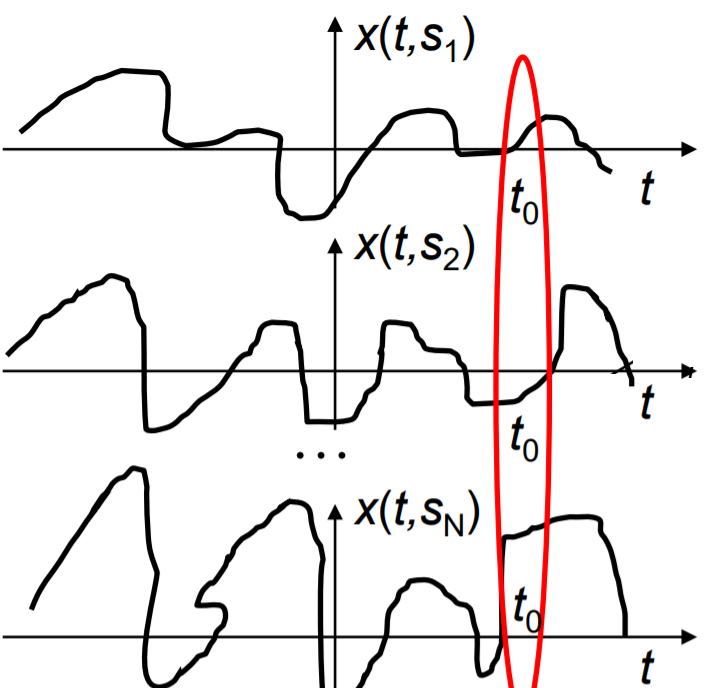
\includegraphics[width=5.5cm]{randomprocesses}
		\caption{scheme to refer while dealing with random processes.} \label{fig:prob:randomprocesses}
	\end{SCfigure} \noindent

	Considering the example in figure \ref{fig:prob:randomprocesses}, every function $x(t,s_i)$ is a realization of the stochastic process while instead the set of all the values read at a certain time (red circle) $x(t_0,s_1)$, $\dots$, $ x(t_0,s_N)$ can be regarded as a random variable $X(t_0)$ extracted from the random process.

	With a description of the stochastic process considering the outcomes $X(t)$ of the random variable changing in time, the relationship between 2 or more random variables $X(t_n)$, $\dots$,  $X(t_s)$ is described by the \textbf{joint probability density function} $f_{pd,X_n\dots X_s}$ for continuous RV or using the joint probability mass function in the discrete-time case.
	
	A complete statistical description of a stochastic process requires to know the joint PDF/PMF of $X(t_n),\dots X(t_s)$ for any tuple of timestamps $(t_n,\dots, t_s)$ and this relations are in general very difficult to be determined.\\
	A weaker condition that allows to describe a random process is instead by knowing the $M^{th}$ order statistic of the joint PDF/PMF of any tuple of random variables $X(t_n),\dots, X(t_s)$ with size $n \leq M$; also those computation can quickly escalates, but in practise with $M=2$ the associated description of the random phenomenon is quite good. The joint CDF for the case $M=2$ is so
	\begin{equation}
		\begin{aligned}
		f_{cd,X_nX_m} (x_n,x_m) & =  \left\{ \begin{aligned}
			& \int_{-\infty}^x \int_{-\infty}^y f_{pd, X_nX_m} (x_n,x_m)\, dx_n\, dx_m && \text{continuous r.v.}\\
			& \sum_j^y \sum_i^x p_{X_{n_i}X_{m_j}} && \text{discrete r.v.}
		\end{aligned} \right. \\
		P\big\{ X(t_n) \leq x, X(t_m) \leq y \big\} & =
		\end{aligned}
	\end{equation}
	If the random variables extracted by the stochastic process are statistically independents then the marginal distribution of each random variable doesn't effect the PDF of the other and in particular we have that
	\begin{equation}
		f_{pd,X_n\dots X_s} (x_n\dots, x_s) = f_{X_n}(x_n) \dots f_{X_s}(x_s) 
	\end{equation}
	
	\paragraph{Example of stochastic process} Let's consider now the random process defined by the random variable
	\[ X(t) = A \cos(\Omega_0 t + \Theta) \]
	where $\Omega_0 \in \mathds R$ is a constant parameter while instead $\Theta$ is another random variable uniformly distributed in the range $[0,2\pi]$ having so the following probability density function:
	\[ f_{pd,\Theta}(\theta) = \begin{cases}
		\frac 1 {2\pi} \qquad & \theta\in[0,2\pi] \\ 0 & \textrm{otherwise}
	\end{cases} \]
	In this case $X(t)$ is a random process: it has a analytical description defined by the cosine function $g(t,\Theta) = \cos(\Omega_0t + \Theta)$ but also has a stochastic contribution depending on the random value of the phase $\Theta$. 
	
	Considering this problem, the goal is to define the probability density function $f_{pd,X}(x(t))$ of the stochastic process, the mean value $\mu(t)$ and the autocorrelation $\phi(t_1,t_2)$ of the function at two different times:
	\begin{enumerate}[a)]
		\item to determine the PDF of the stochastic process we can consider that the argument $\Omega_0 t + \Theta$ of the cosine can be regarded as a unique random variable $\Psi$ uniformly distributed in the range $[0,2\pi]$ for a specific timestamp $t$:
		\[ f_{pd,\Psi}(\psi) = \begin{cases}
			\frac 1 {2\pi} \qquad & \psi\in[0,2\pi] \\ 0 & \textrm{otherwise}
		\end{cases} \]
		Rewriting the random process as $x(t) = A \cos\Psi$, by inverting this equation we can determine the value of the variable $\psi$ as function of the output $x$ as
		\[ \psi= \arccos \left(\frac x A\right) \]
		For every value $x/A$ in the domain $[-1,1]$ such relation gives two solutions in the form $\psi_2 = 2\pi - \psi_1$; knowing so the deterministic function that determines $X$ from the random variable $\Psi$, then the probability density function can be determined using equation \textbf{AGGIUNGERE EQUAZIONE E RIFERIMENTO IN PRECEDENZA} as
		\begin{align*}
			f_{pd,X}(x) & = \sum_{i=1}^2  \frac{f_{pd,\Psi}(\psi_i)}{|g'(\psi_i)|} = \frac 1 {2\pi} \frac{1}{A \sin \psi_1} + \frac 1 {2\pi} \frac{1}{A \sin \psi_2} \\
			& = \frac{1}{2\pi A \sin\left(\arccos \frac x a\right)} + \frac{1}{2\pi A \sin\left(2 -\arccos \frac x a\right)} 
			= \frac1{2\pi A} \left( \frac 1 {\sqrt{1- \left( \frac x A \right)^2 }} + \frac 1 {\sqrt{1- \left( \frac x A \right)^2 }} \right) \\ & = \frac 1 {\pi A\sqrt{1- \left( \frac x A \right)^2 }}
		\end{align*}
		where $g(\psi) = A  \cos(\psi)$ and the property $\sin(\arccos x) = \sqrt{1-x^2}$ has been considered. We can now see that the probability density function can be computed  only when $|x|\leq A$ and in particular
		\[ f_{pd,X}(x) = \begin{cases}
			\frac 1 {\pi \sqrt{A^2-x^2}} \qquad & |x| \leq A \\
			0 & |x|>A
		\end{cases} \]
		Observing that $\Psi$ doesn't depend on time, the PDF of the random variable $X$ isn't either.
		
		\item The mean value of the random process can be trivially calculated by using the first raw statistical moment on the yet found probability density function:
		\[ \mu(t) = \mu = \intinf x f_{pd,X}(x)\, dx = 0 \]
		due to the symmetry of the PDF. The same result could have been obtained considering the deterministic function that related the dependent random variable $X$ with the independent one $\Psi$ using equation \textbf{AGGIUNGERE EQUAZIONE E RIFERIMENTO}:
		\[ \mu = \intinf g(\psi) f_{pd,\Psi}(\psi) \, d\psi = \int_0^{2\pi} A \cos\psi \frac{2 }{2\pi} \, d\psi = \frac A {2\pi} \sin \psi \Big|_{0}^{2\pi} = 0 \]
		
		\item The autocorrelation $\phi(t_1,t_2)$ can be instead calculated using the first order raw statistical moment on two random variables $X(t_1),X(t_2)$ extracted at two different times:
		\begin{align*}
			\phi_X(t_1,t_2) & = E\big\{ A \cos \big(\Omega_0 t_1 + \theta \big) A \cos \big(\Omega_0 t_2 + \theta \big) \big\}
		\end{align*}
		using the linearity property of the expectation operator $E\{\cdot\}$ and using the trigonometric expansion $\cos \alpha \cos \beta = \frac 1 2 \cos(\alpha + \beta) + \frac 1 2 \cos(\alpha - \beta)$ we have		
		\begin{align*}
			\phi_X(t_1,t_2) & = A^2 \, E\left\{ \frac 1 2 \cos \Big( \Omega_0(t_1-t_2) \Big) + \frac 1 2 \cos \Big( \Omega_0 (t_1+t_2) + 2\theta \Big) \right\} \\
			& = \frac {A^2}2 \cos\Big(\Omega_0 (t_1-t_2)\Big) + \frac {A^2}2 \cancelto{0}{E \left\{\cos \Big( \Omega_0 (t_1+t_2) + 2\theta \Big) \right\} }
		\end{align*}
	\end{enumerate}
	
	\subsection{Classification of stochastic processes: stationary cases}
		\paragraph{Strict-sense stationary} As previously seen, a stochastic process can be regarded as a collection of random variables that might change over time; every time a random process has all joints PDF/PMF that are time invariant, then it's defined as \de{strict-sense stationary} and it has that
		\[ f_{pd, X_n} (x_n) = f_{pd,X_{n+k}} (x_{n+k}) \quad \textrm{and} \quad f_{pd, X_n X_m} (x_n, x_m) = f_{pd,X_{n+k}X_{m+k}} (x_{n+k}, x_{m+k}) \qquad \forall k \]
		Having that the probability density function (or the PMF in the discrete case) is always constant over time it descent that also all the properties of the distribution (such mean $\mu$ and variance $\sigma^2$) are constant. Having strict-sense stationary processes is usually impossible in real life and happens only upon strong theoretical hypothesis; for engineering applications most processes are however approximated as strict-sense stationary.
		
		\paragraph{Wide-sense stationary} A process is instead defined as \de{wide-sense stationary} if just the mean of any random variable extracted from the process itself is independent from the time and the correlation depends just on the  time difference between the pair of random variables, so:
		\begin{align*}
			& \mu_n = E\{ X(t_n) \} = \mu = \textrm{constant} \\
			& \phi_X (t_n,t_m) = E\{ X(t_n) X(t_m) \} = \phi_X \big(t_n-t_m\big) \qquad \forall t_n,t_m
		\end{align*}
		
		From this definition we can see that a strict-sense stationary process it's also wide-sense stationary, while the contrary isn't true in general. \\
		We define as \textbf{autocorrelation} $\phi_X$ the correlation between random variables extracted from the same stochastic process, while if they came from different random processes the correlation is called \textbf{cross-correlation}. For wide-sense stationary processes we have the following properties for the autocorrelation:
		\begin{align*}
			i) \qquad & \phi_X (t_m) = \phi_X (-t_m) && \forall t_m \\
			ii) \qquad & \phi_X(0) = E\{ X^2(t_m)\} && \forall t_m \\
			iii) \qquad & |\phi_X(t_m)| \leq \phi_X(0)
		\end{align*}
		
		\paragraph{Cyclo-stationarity} A stochastic process is defined as \de{cyclo-stationary} (with period $T_0$) iw both mean $\mu$ and autocorrelation $\phi$ are periodic with period $T_0$, so
		\begin{align*}
			i) \qquad & \mu(t+ kT_0) = \mu(t) && \forall k\in\mathds Z \\
			ii) \qquad & \phi_X(t+\tau+kT_0, t+kT_0) = \phi_X(t+\tau,t) && \forall \tau \in \mathds R , \ \forall k\in \mathds Z
		\end{align*}
		Example of cyclo-stationary random process is $Y(t) = X(t) \cos(\Omega_0 t)$ where $X(t)$ is a wide-sense stationary stochastic process; the related period is $T_0 = 2\pi \Omega_0$.
		
		\paragraph{Ergodicity} Given a strictly-sense stationary process $X(\cdot)$, for any deterministic function $g(X)$ it's possible to defined the \textbf{ensemble} (statistical) \textbf{average} defined as
		\begin{equation}
			E\big\{ g\big(X(t)\big) \big\} = E\{g(x)\} = \intinf g(x) f_{pd,X}(x)\, dx
		\end{equation}
		where the result is time invariant due to the stationarity of the starting process; we can also compute the \textbf{time average} of the $i$-th realization of the stochastic process as
		\begin{equation}
			\big\langle g\big(x(t,s_i)\big) \big \rangle = \lim_{T\rightarrow \infty} \frac 1 T \int_{-\frac T 2}^{\frac T2} g\big( x(t,s_i) \big)\, dt 
		\end{equation}
		
		With those definition a strict-sense stationary process $X(\cdot)$ is defined as \de{ergodic} if it's ensemble average is equal to the time average of it's each realization, so if
		\[ \big\langle g\big(x(t,s_i)\big) \big \rangle = E\{g(X)\} \hspace{2cm} \forall s_i \in S \textrm{ and } \forall g(\cdot) \]
		As consequence of this definition the statistical moment of the random process can be estimated from a single and sufficiently long ($T$ \textit{big}) realization of the process itself:
		\begin{equation}
		\begin{aligned}
			\mu = E\{X\} & = \frac 1 T \int_{-\frac T 2}^{\frac T2} x(t,s_i)\, dt \\
			P_X = E\{X^2\} & = \frac 1 T\int_{-\frac T 2}^{\frac T2} x^2(t,s_i)\, dt \\
			\phi_X(\tau) & = \frac 1T\int_{-\frac T 2}^{\frac T2} x(t,s_i) x(t+\tau, s_i)\, dt
		\end{aligned}
		\end{equation}
		where $P_X$ is the power of the random process.
		
		\paragraph{Energy and power for random signals} Given a random process $X(t)$ with realizations $x(t,s_i)$, for each of them its possible to compute it's energy $\mathcal E_i$ and power $\mathcal P_i$ as
		\begin{equation}
			\mathcal E_i = \intinf x^2(t,s_i)\, dt \hspace{2cm} \mathcal P_i = \lim_{T\rightarrow \infty} \frac 1 T \int_{-\frac T2}^{\frac T2} x^2(t,s_i)\, dt
		\end{equation}
		For each realization the values $\mathcal E_i,\mathcal P_i$ are deterministic, however considering the whole random process they themselves can be described by a non-deterministic stochastic variable with  associated statistical distribution. We can so compute the \de{energy} $E_x$ and the \de{power} $E_x$ of the random process has the expected value of the energies/powers random variables, so
		\begin{equation}
		\begin{aligned}
			E_X & = E\{\mathcal E \} = E\left\{ \intinf X^2(t)\, dt \right\} = \intinf E\{X^2(t)\}\, dt = \intinf \phi_X^2(t,t)\,dt \\
			P_X & = E\{\mathcal P\} = \lim_{T\rightarrow\infty} \frac 1 T \int_{-\frac T2}^{\frac T  2} \phi_X^2(t,t)\, dt
		\end{aligned}
		\end{equation}
		
		In the case of wide-sense stationary processes we have that $\phi_X(t)$ is constant and (unless $X(t) = 0$) we have a divergent energy for the signal and a constant power equal to
		\[ E_X = \intinf \phi_X(0) \,dt \rightarrow \infty \hspace{3cm} P_X = \phi_X^2(0) \]
		In this case we can so state the $X$ is just a \textbf{power signal}.
		
	\subsection{Power spectral density} \label{sec:prob:psd}
		Considering a wide-sense stationary random process, any pair $X(t), X(t+\tau)$ of random variables extracted tends to be uncorrelated when the temporal distance $\tau$ between them grows. Observing that the autocorrelation sequence has typically a finite energy and is sometimes also absolutely summable, then it's possible to compute the Fourier transforms of the autocorrelation for both the continuous and discrete time case:
		\begin{equation} \label{eq:prob:psd}
		\begin{aligned}
			\Phi_X(\Omega) & = \intinf \phi_X(t) e^{-j\Omega t} \, dt \qquad && \text{: continuous time case} \\
			\Phi_X(e^{j\omega}) & = \infsum m \phi_X(m) e^{-j\Omega m} \, dt \qquad && \text{: discrete time case} \\
		\end{aligned}
		\end{equation}
		Knowing that $\phi(\tau)$ is an even real-evaluated function, then $\Phi_X(\Omega)$ is also positive; the spectrum $\Phi_X$ is more frequently referred as the \de{power spectral density} of the signal due to the fact that the power of the signal can also be computed as
		\begin{equation}
			P_X = \frac 1 {2\pi} \intinf \Phi_X(\Omega)\, d\Omega
		\end{equation}
		
		
		
		\paragraph{White noise} \textbf{AGGIUNGERE IL WHITE NOISE}
		
	
	
	
	